\section{Exploratory Data Analysis (EDA): A Simple Overview}

Exploratory Data Analysis (EDA) is the process of investigating and summarizing a dataset before jumping into more formal analysis or modeling. It helps us understand the data’s structure, detect patterns, and spot any issues like missing values or outliers. EDA uses statistical summaries and visual tools to gain insights, making it easier to build more accurate models later.

\subsection*{Types of Exploratory Data Analysis}

\subsubsection*{Univariate Analysis}  
This phase focuses on analyzing individual variables to understand their characteristics. Common techniques include:
\begin{itemize}
    \item Histograms: To visualize data distribution.
    \item Box Plots: For detecting outliers.
    \item Summary Statistics: Such as mean, median, mode, variance, and standard deviation.
\end{itemize}

\subsubsection*{Bivariate Analysis}  
Bivariate analysis examines relationships between two variables to identify correlations or dependencies. Techniques used include:
\begin{itemize}
    \item Scatter Plots: To visualize relationships between continuous variables.
    \item Correlation Coefficient: To quantify the strength of relationships.
    \item Cross-tabulation: For categorical variables.
\end{itemize}

\subsubsection*{Multivariate Analysis}  
This phase involves analyzing more than two variables simultaneously to explore complex interactions and relationships within the dataset. Common techniques include:
\begin{itemize}
    \item Pair Plots: To visualize pairwise relationships between multiple variables.
    \item Principal Component Analysis (PCA): To reduce the dimensionality of the data while retaining the most important features.
    \item Multiple Regression: To understand the relationship between one dependent variable and multiple independent variables.
\end{itemize}

\subsection*{Steps for Performing Exploratory Data Analysis (EDA)}

\begin{enumerate}
    \item \textbf{Understand the Problem and the Data:} First, we try to understand what the dataset is about and what questions we want to answer. For example, in climate data, we might want to know how temperature changes over months.
    
    \item \textbf{Import and Inspect the Data:} We load the data into tools like RStudio or Google Colab. Then, we inspect the structure — checking the number of rows, types of variables (numeric, categorical), and basic statistics like mean, median, and range.
    
    \item \textbf{Handle Missing Data:} Missing values are common in real-world data. We can handle them by techniques such as:
    \begin{itemize}
        \item Removing rows with missing values.
        \item Filling missing entries using mean, median, or mode (called imputation).
        \item Using more advanced methods like interpolation or prediction models.
    \end{itemize}
    
    \item \textbf{Explore Data Characteristics:} We perform basic statistical analysis to understand each variable. For example:
    \begin{itemize}
        \item Calculate mean, median, variance, and standard deviation.
        \item Create histograms and box plots to check data distribution and spot outliers.
    \end{itemize}
    
    \item \textbf{Perform Data Transformation:} Sometimes we need to adjust the data to make analysis easier. Common transformations include:
    \begin{itemize}
        \item Normalization: Scaling values between 0 and 1.
        \item Standardization: Adjusting data to have a mean of 0 and standard deviation of 1.
        \item Aggregation: Summarizing data, like taking the average monthly temperature from daily values.
    \end{itemize}
    
    \item \textbf{Visualize Data Relationships:} Visualization helps us see patterns that are hard to find in tables. We use:
    \begin{itemize}
        \item Scatter Plots: To explore relationships between two continuous variables.
        \item Bar Charts: To compare categories.
        \item Heatmaps: To visualize correlations among multiple variables.
        \item Line Charts: To show trends over time, especially in climate data.
    \end{itemize}
    
    \item \textbf{Handle Outliers:} Outliers are values that are much higher or lower than most data points. We can:
    \begin{itemize}
        \item Analyze if they are genuine observations.
        \item Correct or remove them if they are due to errors.
    \end{itemize}
    
    \item \textbf{Communicate Findings and Insights:} After analyzing the data, we summarize the key points through reports, graphs, and presentations. Clear communication makes the results understandable to everyone, even those who are not data experts.
\end{enumerate}

\begin{figure}[h]
\centering
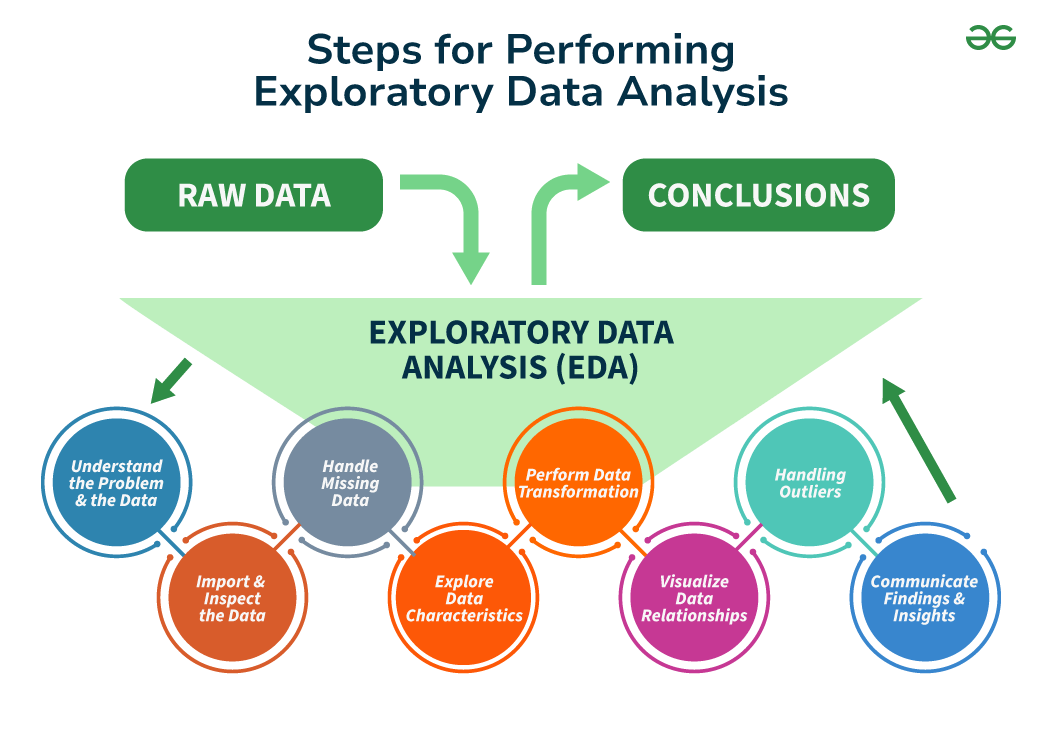
\includegraphics[width=0.6\textwidth]{figures/eda.png}
\caption{Steps of Performing EDA }
\end{figure}
For instance, if we want to explore climate data using Exploratory Data Analysis (EDA), we begin by loading the climate data, such as daily temperatures, into an analysis environment. The first step is to inspect the data for any missing values or errors. Next, we analyze the temperature distribution using histograms to determine whether the weather is mostly warm or cool. We also examine the relationship between temperature and other variables, like humidity, using scatter plots. In more complex cases, we explore how multiple factors, such as temperature, humidity, and wind speed, interact with each other. If we find missing data, we can either remove the affected entries or replace them with average values. Based on our analysis, we might identify trends, like rising temperatures over time, which could suggest climate change. Finally, we use visual tools such as scatter plots and heatmaps to clearly illustrate these relationships and communicate our findings. 
In this book, we will dive deeper into how to analyze climate data using these methods and explore additional techniques to uncover meaningful insights from real-world climate datasets.

